% This is samplepaper.tex, a sample chapter demonstrating the
% LLNCS macro package for Springer Computer Science proceedings;
% Version 2.20 of 2017/10/04
%
\documentclass[runningheads]{llncs}
%
\usepackage{graphicx}
\usepackage{amsmath,epsfig}
% \usepackage{caption}
\usepackage{float} 
% \usepackage{subcaption}
\usepackage{multirow}
\usepackage{hyperref}
\usepackage{marvosym}
\usepackage{svg} % 需使用包
% Used for displaying a sample figure. If possible, figure files should
% be included in EPS format.
%
% If you use the hyperref package, please uncomment the following line
% to display URLs in blue roman font according to Springer's eBook style:
% \renewcommand\UrlFont{\color{blue}\rmfamily}



\pagestyle{empty}

\begin{document}
%
\title{ER-SFM: EFFICIENT AND ROBUST CLUSTER-BASED STRUCTURE FROM MOTION\thanks{Supported by the Open Fund of Science and Technology on Parallel and Distributed Processing Laboratory (PDL), WDZC20235250106.}}

%\titlerunning{Abbreviated paper title}
% If the paper title is too long for the running head, you can set
% an abbreviated paper title here
%
% \author{Anonymous PRCV submission}

\author{Zongxin Ye \and
Wenyu Li \and
Sidun Liu \and
Peng Qiao\textsuperscript{(\Letter)} \and
Yong Dou
} 

%
% \authorrunning{F. Author et al.}
% First names are abbreviated in the running head.
% If there are more than two authors, 'et al.' is used.
%
% \institute{National Key Laboratory of Parallel and Distributed Computing, National University of Defense Technology, Changsha 410000, China }
\institute{National Key Laboratory of Parallel and Distributed Computing, College of Computer, National University of Defense Technology, Changsha, China
\email{
\{yezongxin21,wenyu18,liusidun,pengqiao,yongdou\}@nudt.edu.cn}}

% {College of Computer Science and Technology, National University of Defense Technology, Changsha 410073, China };
% National Key Laboratory of Parallel and Distributed Computing, National University of Defense Technology, Changsha 410073, China,pengqiao@nudt.edu.cn

\maketitle              % typeset the header of the contribution

\begin{abstract}
Structure from Motion~(SfM) is a fundamental computer vision technique that recovers scene structure and camera motion from multi-view images. When facing large-scale scenarios, cluster-based methods are commonly employed to improve reconstruction efficiency. However, these methods currently face challenges regarding their limited robustness, redundant computation, and drift. To address these issues, we propose a unified pipeline called ER-SfM, which enhances the three key aspects of cluster-based SfM: image clustering, local reconstruction, and merging. In terms of image clustering, we propose a three-stage image clustering method to ensure adequate and reliable connections between clusters. In the local reconstruction stage, we expedite the reconstruction process by eliminating duplicate point cloud computation. In the final merging stage, we introduce a global merging algorithm without scale ambiguity to address the drift problem. Extensive experimental results demonstrate the superior performance of our method in terms of both robustness and efficiency compared to state-of-the-art methods.

\keywords{Parallel Structure from Motion \and 3D Reconstruction \and Image Clustering \and Global Averaging.}
\end{abstract}


\section{Introduction}

Structure from Motion~(SfM) is a vital process in computer vision that retrieves camera poses and scene point clouds from multiple images. It serves as a critical step for various computer vision tasks, including Neural Radiance Fields~\cite{Cnerf}, Multi-View Stereo ~\cite{RayMVSNet,RayMVSNet++}, and 3D Gaussian Splatting~\cite{3DGS}.

To tackle the efficiency challenge posed by large-scale scenarios, numerous cluster-based methods~\cite{AccPara,AdaSfM,Divide_conquer,TC-SfM,gsfm,large_averaging,merge} have been proposed. Typically, these methods utilize images as nodes and construct a connected graph according to the number of feature matches between images, denoted as \textbf{image graph}. Subsequently, the image graph is partitioned into clusters via a graph cut algorithm~\cite{NCUT}.To facilitate cluster merging, it is typically necessary to expand additional common images within the clusters. Afterwards, clusters are processed in parallel for incremental SfM. Finally, the clusters are merged by utilizing the similarity transformations calculated from the common images shared between them.

\textbf{Image clustering, local SfM, and merging} are three key components of parallel incremental methods, which directly impact the robustness and efficiency of the system. 

\begin{figure}[t]
\centerline{\includegraphics[width=1\textwidth]{figs/compare_20K.pdf}}
	\caption{ Reconstructions generated from the Aerial-20k dataset (23458 images). Our method only takes 1.5 hours, while GraphSfM takes 7.5 hours.}
	\label{Aerial-20k}
\end{figure}

1) \textbf{Image clustering}. 
Expanded common images are critical to the merging of adjacent clusters. Nonetheless, too many common images increase reconstruction and merging time. To decrease redundant common images and improve the merging efficiency, current methods~\cite{gsfm,AccPara,AdaSfM} limit the number of common images within a cluster and simplify the connected graph. However, these methods do not decouple the impact of common images on efficiency and connectivity, thus often compromising connectivity while pursuing efficiency, as illustrated in Fig.~\ref{fig_cluster_graph}.

2) \textbf{local SfM}.
Current image expansion methods~\cite{gsfm,Divide_conquer,AdaSfM,AccPara}  rely solely on image matches or similarity without considering the correlation with the entire cluster. The common images expanded in these methods lack reliability. Moreover, these expansion images are typically registered using incremental SfM, which entails point cloud reconstruction and repeated Bundle Adjustment, significantly diminishing efficiency. In fact, the point clouds corresponding to these expansion images will be reconstructed in multiple clusters, resulting in a large number of unnecessary duplicate calculations.

\begin{figure}[t]
    \centering
        \includegraphics[width=0.8\textwidth]{figs/cluster_graph.pdf}
	\caption{Cluster graphs for Lund Cathedral dataset when cluster size is 30.}
    \label{fig_cluster_graph}
\end{figure}

3) \textbf{Merging}. Existing merging methods~\cite{gsfm,Divide_conquer,AdaSfM,merge,TC-SfM} are mainly path-based. Although minimized by selecting the optimal path to some extent, the cumulative error persists, and the drift problem~\cite{Drift} remains unavoidable, as shown in Fig.~\ref{fig_cluster_size}(a). Furthermore, incorrect selections of duplicated point clouds and camera poses introduce additional errors.

To tackle the problems above and systematically improve efficiency and robustness, we introduce a pipeline, named Efficient and Robust Structure from Motion, coined as ER-SfM. This pipeline focuses on refining the three core stages of parallel incremental SfM, as shown in Fig.~\ref{fig_pipeline}. At \textbf{Image clustering} stage, to decouple the impact of common images on efficiency and connectivity, we determine the common image in two phases. Firstly, instead of expanding the images from a part of selected cluster edges, we expand all images to restore all the connections without limitation on the number of expanded images within each cluster. Secondly, to maintain the connectivity while improving efficiency, we filter the common images between each pair of clusters instead of removing cluster edges directly. As shown in Fig.~\ref{fig_cluster_graph}(b), our image clustering strategy maintains connectivity. At \textbf{Local SfM} stage, To enhance reliability, we perform local incremental SfM on the cluster before the expansion step (Fig. \ref{fig_pipeline}), and then filter expansion images in light of the visibility of the reconstructed point cloud. In order to reduce redundant calculations, we only restore the poses of the expansion images through the perspective-three-point (P3P)\cite{P3P}. At \textbf{Merging} stage, we replace the path-bathed method by proposing a global algorithm to handle the drift problem. However, global methods often face scale ambiguity~\cite{mvg}. Therefore, we use the results of local reconstruction to decouple scale and translation. In addition, we facilitate the correct selection of duplicate elements by considering both the reprojection error and the number of point cloud observations.

The evaluation on multiple datasets shows that ER-SfM is significantly more robuster than state-of-the-art clustering-based method while also achieving a speedup of 2-9 times. Fig.~\ref{Aerial-20k} illustrates the reconstruction outcomes of a very large-scale scene, demonstrating the faster reconstruction speed and superior performance of our method.

\section{RELATED WORKS}
SfM methods are commonly categorized into two categories: incremental methods~\cite{mvg,colmap} and global methods~\cite{Revisiting_ra}. Incremental approaches register images one by one, and continuously optimize the camera poses and point cloud using Bundle Adjustment(BA) throughout the process. This makes the incremental approaches more robust and accurate while less efficiency. Additionally, although the incremental approaches typically adopt additional re-triangulation step to mitigate cumulative errors, they are still prone to drift problem. Global approaches simultaneously recover the camera poses of all images by solving rotation and translation averaging problem. Considering all images simultaneously improves the efficiency and leads to no drift. However, global methods are sensitive to outliers, and solving the translation averaging problem is challenging due to scale ambiguity. Moreover,the time and spatial complexity of Global methods is cubic and square respectively in the number of input images. 

Due to efficiency constraints, both incremental and global approaches are difficult to handle large-scale scenarios. Certain cluster-based methods leverage parallel computing to enhance efficiency. Bhowmick et al.~\cite{Divide_conquer} attempted to solve large-scale SfM using a divide-and-conquer approach. They employed a graph cut algorithm~\cite{NCUT} to partition the images into different clusters. Then each cluster is reconstructed separately, enabling a parallel implementation. Finally, the reconstructed clusters were merged into a unified coordinate system. 
However, the merging algorithm overlooked the issue of drift caused by accumulated errors. To mitigate the errors, some studies~\cite{TC-SfM,merge} employed minimum spanning trees (MST) to identify the optimal merging path. GraphSfM~\cite{gsfm} further reduces merging errors by exploiting an additional minimum height spanning tree. However, these path-based merging methods cannot fundamentally avoid drift issues. To eliminate drift, some studies~\cite{AccPara,large_averaging,AdaSfM} introduce global methods into cluster-based methods. Zhu et al.~\cite{AccPara} utilizes the results of local reconstruction for motion averaging to re-estimate the poses and reconstruct the point cloud. However, this approach entails significant repeated computation. This approach was further improved in a later work~\cite{large_averaging}, which introduces a block-wise global method that iteratively applies local motion averaging and global motion averaging. Nevertheless, it faces the challenge of scale ambiguity. AdaSfM~\cite{AdaSfM} performs coarse global SfM to regularize and align the results of local incremental SfM, but this coarse global SfM requires additional sensor measurements as inputs. 

\section{METHODOLOGY}

The pipeline of ER-SfM is shown in Fig.~\ref{fig_pipeline}. Initially, features and matches are extracted from the images. Then, the images are partitioned into clusters for separate reconstruction. The resulting reconstructions from all clusters are then merged. Finally, a global BA is executed to get obtain final result. To enhance the robustness and efficiency, we optimized three key steps of cluster-based method: image clustering, local SfM, and merging. Each of these steps will be elaborated in subsequent subsections.

\begin{figure}[t]
    \centering
        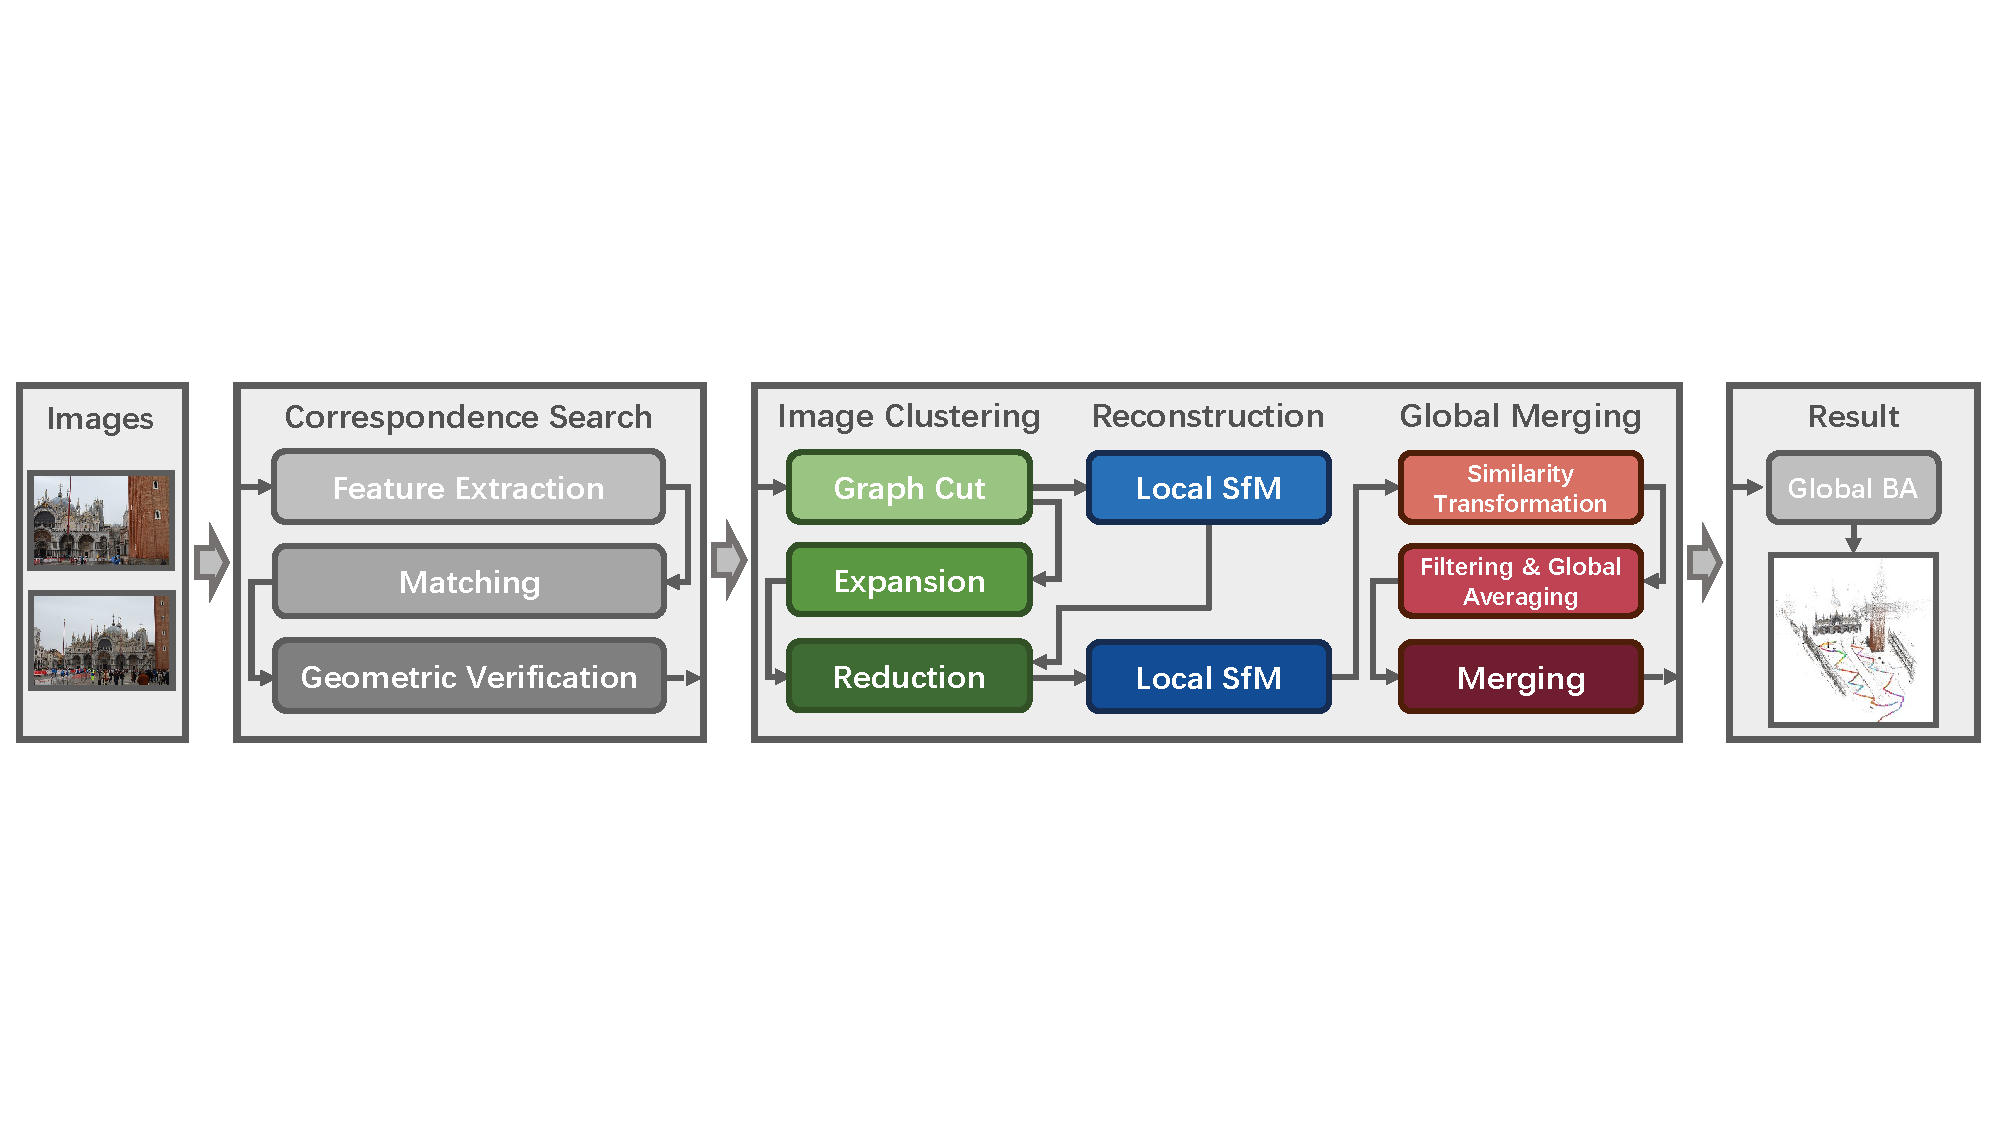
\includegraphics[width=1\textwidth]{figs/pipeline.pdf}
        \caption{Pipeline of ER-SfM.}
    \label{fig_pipeline}
    \vspace{-0.5em}
\end{figure}

\subsection{Image Clustering}
As shown in Fig.~\ref{fig_image_clustering}, our image clustering algorithm is divided into three stages: graph cut, expansion, and reduction. We will detail each step as follows.

\textbf{Graph Cut}. In this step, we first build a connected graph named \textbf{image graph} based on images and feature matches. In the graph, each node represents an image, while the weight on each edge represents the number of matches. In this way, the image clustering problem is converted into a graph cut problem (Fig.~\ref{fig_image_clustering}(a)). As with some previous approaches\cite{gsfm,Divide_conquer,AccPara}, we use the NCuts\cite{NCUT} algorithm to solve this problem.

\begin{figure}[t]
    \centering
        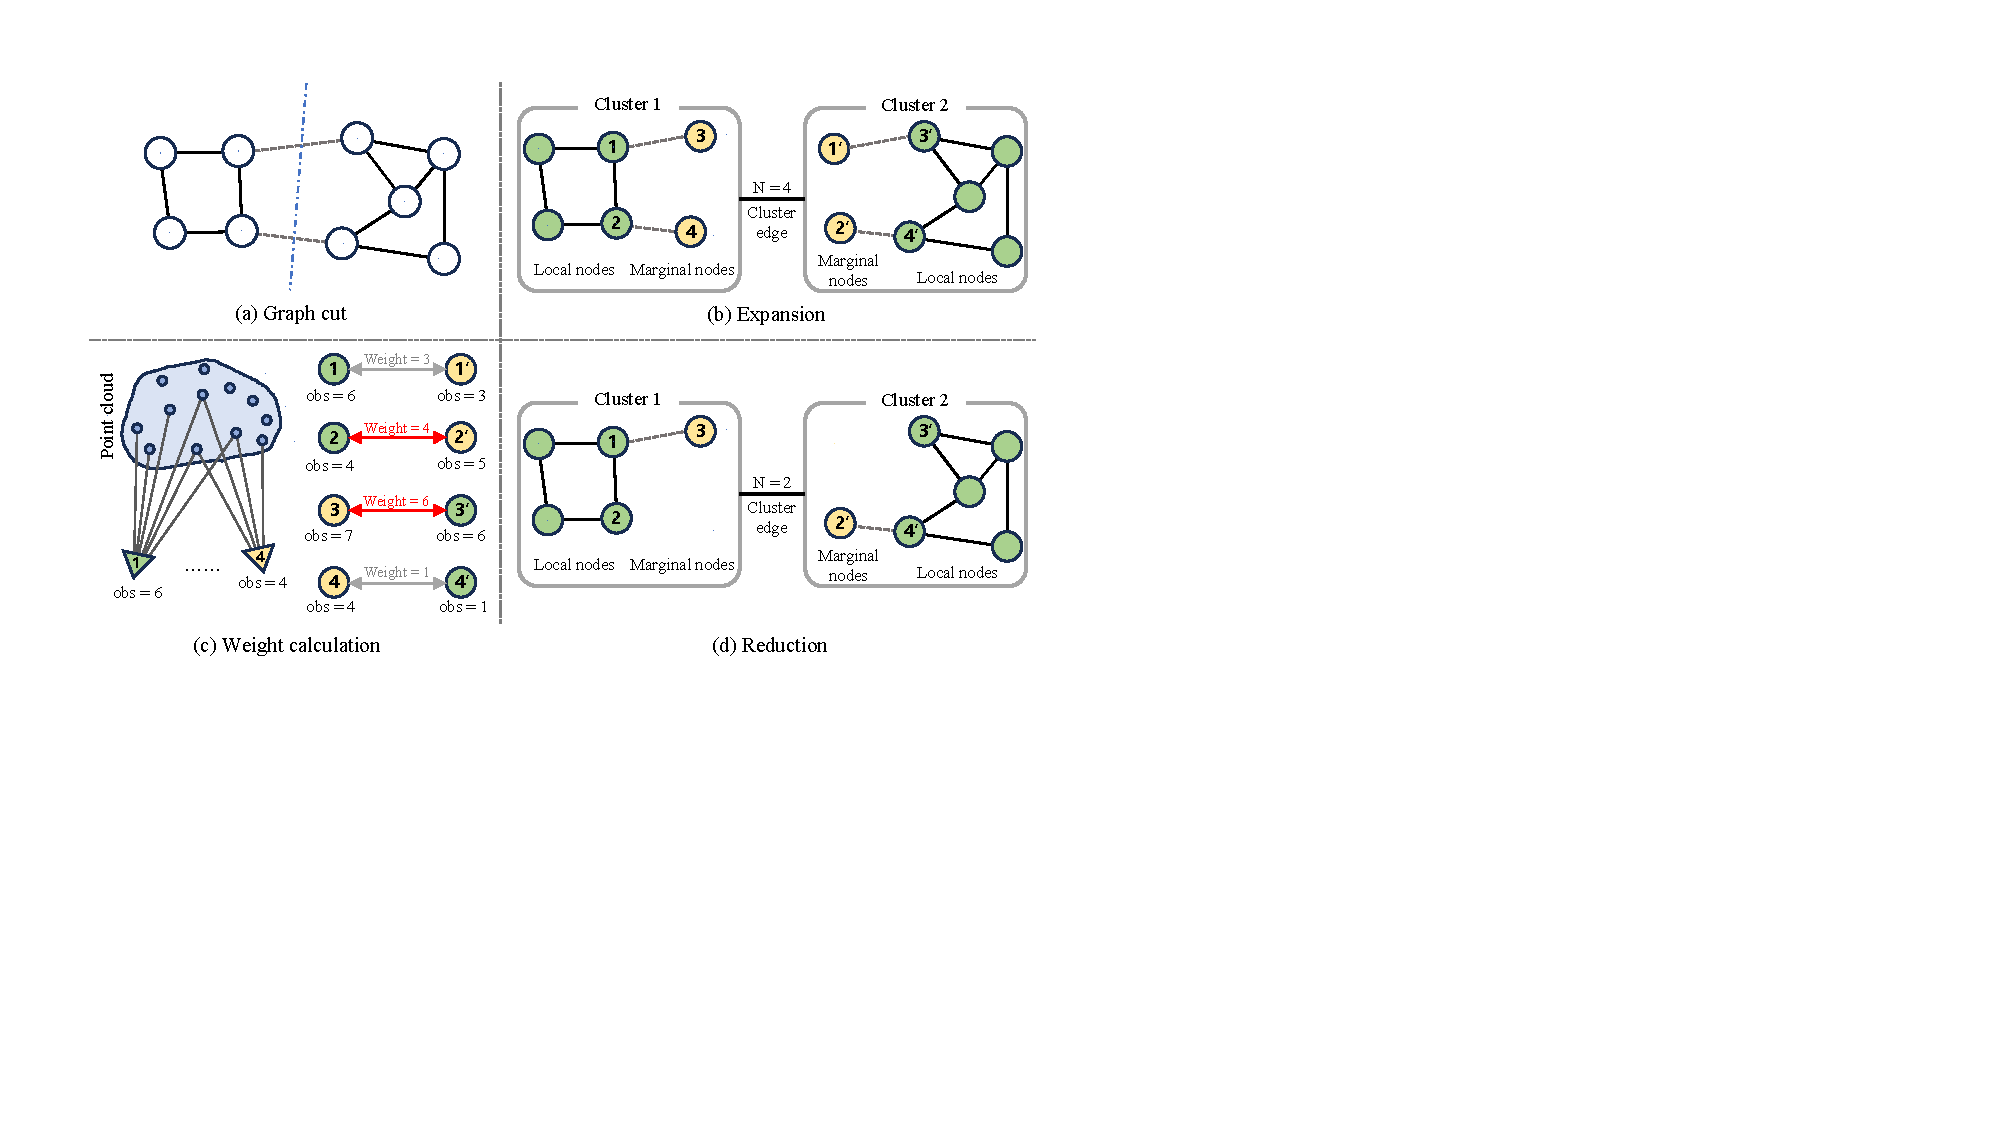
\includegraphics[width=0.99\textwidth]{figs/cluster_pipe.pdf}
        \caption{Pipeline of image clustering. (a) Graph cut. Nodes are depicted as circles, edges as dashed lines, and lost edges as dotted lines. (b) Expansion. In each cluster, local nodes are labeled in green, marginal nodes are labeled in yellow. The common images shared between clusters are assigned the same number. $N$ represents the weight of cluster edge. (c) Weight calculation. triangles represent the cameras corresponding to the images. $obs$ indicates the number of points observed. The double arrows indicate the common image, where the weight is the minimum $obs$ among the common images. (d) Reduction. Retain selected common images.}
    \label{fig_image_clustering}
    \vspace{-0.5em}
\end{figure}

\textbf{Image Expansion}. To establish connections between clusters, we expand common images to these clusters. The edges that are cut off during graph cut step are referred to as \textbf{lost edges}. The images connected by each lost edge belong to two different clusters. For each cluster, all the lost edges connected to it are collected and all images that connected to these lost edges are expanded. The images that are clustered during graph cut step are called \textbf{local images}, while the images that are added at expansion step are called \textbf{marginal images}. This can be seen in Fig.~\ref{fig_image_clustering}(b). In subsequent local reconstruction stage, the point cloud reconstruction for marginal images can be skipped to improve processing speed.

\textbf{Image Reduction}. We construct a \textbf{cluster graph} with cluster as node and the weight $N$ of cluster edge as the number of reliable common images between two clusters. Since local images undergo more BA optimization, their poses are deemed more reliable compared to those of marginal images. A common image between two clusters is considered reliable if it is a local image in either of the two clusters.

To reduce the redundancy caused by image expansion and filter out outliers, previous methods~\cite{gsfm,AccPara,AdaSfM} limit the number of marginal nodes within each cluster and only retain the most reliable cluster edges. As shown in Fig.~\ref{fig_cluster_graph}(a), these methods decrease cluster graph connectivity, potentially leading to disconnections. To address this issue, our approach restricts the number of common images within cluster edges instead. In Fig.~\ref{fig_image_clustering}(c), for any image, its weight is the number of reconstruction points that observed within a cluster. Generally, the more observation points, the more reliable the camera pose is. The weight of a common image in a cluster edge is the minimum weight of the image in the two clusters connected by the edge. We set a weight threshold for common images to improve reliability. For each cluster edge, we select the $s$ most weighted common images. Marginal images that are not selected by any cluster edge will be removed from their cluster. To calculate the scale, we remove cluster edges with weight $N<=2$. By image expansion and reduction, we obtain an adequate number of reliable common images for subsequent merging step. Determining the common image through our extension and reduction steps can decouple the effect of the common image on efficiency and connectivity. Thus, efficiency and connectivity can be ensured simultaneously.

\subsection{Local Parallel Reconstruction}
To improve robustness, we employ incremental SfM for our local reconstruction. We observe that the point cloud derived from local images assists in selecting common images during the reduction step, while marginal images solely serve to connect clusters, as their corresponding point clouds are reconstructed in other clusters. To address this, we divide the local reconstruction into two stages alternating with image clustering. The first stage is executed before image reduction, involving the reconstruction of poses and point clouds for all local images. In the second stage, following image reduction, we exclusively employ the P3P~\cite{P3P} to calculate poses for marginal images. It is worth noting that certain methods~\cite{AccPara,AdaSfM} do not guarantee direct connections between all marginal images and the local images. Therefore, the point cloud of some expansion image needs to be reconstructed to assist in restoring the poses of other marginal images. 


\subsection{Cluster Merging}

We finally present a robust and accurate merging algorithm. The key aspect lies in employing global approach to eliminate drift and leveraging the relative scale of clusters to resolve the scale ambiguity problem encountered during global SfM approaches.

\textbf{Similarity Transformation.} We define the subscript $ij$ of the similarity transformation as the transformation from $j$ to $i$. Relative rotation, translation, and scale are denoted as $R_{ij}$, $t_{ij}$, and $s_{ij}$, respectively. By aligning the common images between clusters, we compute the similarity transformation for each cluster edge. We adopt the method introduced in GraphSfM~\cite{gsfm} to compute the relative scale $s_{ij} = {(C_j^{k_1} - C_j^{k_2})} / {(C_i^{k_1} - C_i^{k_2})}$, where $C_i^k$ represents the center of camera $k$ in the coordinate system of cluster $i$. We use 
\begin{align}
R_{ji} &= R_{j}^TR_i \\ 
t_{ji} &= R_{j}^T(s_{ji}t_{i} - t_{j})
\end{align} 
to calculate relative translation and rotation, where $R_{i}$ and $t_{i}$ are the camera poses of the common images. The derivation is shown in the supplementary. Considering that each cluster edge usually corresponds to multiple pairs of common images, RANSAC~\cite{RANSAC} is used to select the best common images to calculate the similarity transformation. 


\textbf{Graph Filtering.} We extend the rotation-based loop constraint~\cite{loop} to scale and translation to filter outliers. Specifically, we validate all triplets. The triplet with a circular error greater than threshold $\epsilon$ is the outlier:
\begin{align}
d(R_{ij}R_{jk}R_{ki},I) > \epsilon_r \\ 
|s_{ij}s_{jk}s_{ki} - 1| > \epsilon_s \\
\frac {3 || s_{ij}R_{ij}t_{ij} + s_{ik}R_{ik}t_{kj} + t_{ik} ||_2} {||t_{ji}||_2+||t_{kj}||_2+||t_{ki}||_2} > \epsilon_t
\end{align} 
Note that the loop constraint for translation is applied after the rotation and scale averaging. Actually, $R_{ji}$ and $s_{ji}$ in equation (5) is based on the result of rotation and scale averaging.

\textbf{Global Averaging.} Global scale $s_i$ and rotation $R_i$ are calculated independently after graph filtering. For scale averaging, we solve the L1 optimization problem for the equation system $s_{ij}s_{j}-s_i=0, i\neq j \ and \ i,j \in0,1,..,N$. Where $N$ is the total number of clusters. Global rotations are computed as done by OpenMVG\cite{mvg}, with a least-square minimization that tries to satisfy equations $R_{ij}R^T_i - R^T_j=0$. Once the global scale and rotation are obtained, the translation averaging no longer has scale ambiguity and can be solved directly via L2 optimization: $R_jt_{ji}-s_{ji}t_i-t_j=0$, where $R_j$ and $s_{ij}$ are obtained by rotation averaging and scale averaging. To remove ambiguity, we set $s_0$, $R_0$ and $t_0$ to 0, identity matrix $I$ and zero vector $0$, respectively.


\textbf{Cluster Merging.} 
According to the result of global averaging, all clusters are merged into cluster $0$. The similarity transformation from cluster $i$ to cluster $0$ is
\begin{align}
R_{0i} &= R^T_0R_i = R_i \\
s_{0i} &= s_0/s_i = 1/s_i \\
t_{0i} &= s_{0i}R_0^Tt_i-R_0^Tt_j
\end{align} 

There may be duplicate camera poses and structure points between different clusters. For the repeated points, we calculate their re-projection errors and retain the smallest. Any point with significantly large re-projection error is considered as outlier. For repeated camera poses, we introduce a reliability metric $m = obs/err$, where obs is the number of observed points and err is the mean reprojection error.



\section{EXPERIMENTS}
\begin{figure}[t]
    \centering
        \includegraphics[width=1\textwidth]{figs/compare_all.pdf}
        \caption{Reconstruction results on public datasets. The Rubble dataset presents two different perspectives. Global OpenMVG (OpenMVG-G) and GraphSfM perform poorly in some datasets, while our approach overcomes these problems. }
    \label{fig_compare_all}
    \vspace{-1.5em}
\end{figure}
We evaluate our algorithm with several datasets: four small scenes (Gerrard Hall, South Building and Person Hall from ~\cite{colmap}, DTU~\cite{DTU}) consisting of sparse images and five large-scale scenes (Lund Cathedral, Duomo and San Marco from ~\cite{Duomo}, Rubble from~\cite{Rubble}, Aerial-20k) . We compare with two widely used incremental SfM apprachs, COLMAP~\cite{colmap} and OpenMVG~\cite{mvg}, and a state-of-the-art cluster-based method, GraphSfM~\cite{gsfm}. Our local reconstruction is conducted via OpenMVG~\cite{mvg}, while other incremental SfM methods also work. More details of the experiment settings can be found in the supplementary.


\begin{table}[h]
\caption{Efficiency and accuracy evaluated on datasets with different scales. $T$ represents the reconstruction time, without final BA. $N_p$, $Err$ represents the number of 3D points and the mean reprojection error, respectively. The best results are highlighted in bold. “-” represents that the result is incorrect.} 
\resizebox{\linewidth}{!}{
\begin{tabular}{|c|c|c|c|c|c|c|c|c|c|c|c|c|c|c|}

\hline

\multicolumn{2}{|c|}{\multirow{2}{*}{dataset}} 
	&	\multirow{2}{*}{images}
	& 	\multicolumn{3}{c|}{COLMAP}
	&	\multicolumn{3}{c|}{OpenMVG}
	& 	\multicolumn{3}{c|}{GraphSfM}
	&	\multicolumn{3}{c|}{Ours}	
	\\
\cline{4-15}

\multicolumn{2}{|c|}{} &{} &$T$ & $N_p$ & $Err$ &$T$ & $N_p$ & $Err$ &$T$ & $N_p$ & $Err$ &$T$ & $N_p$ & $Err$ \\
\hline

\multicolumn{2}{|c|}{Gerrard Hall}
        %images %T(COL) err     T(MVG_I) ERR          T(G) ERR    T(O)         ERR
	&100  	&105    &58261 	  &1.08	    &151	&99195    &0.26   	&131    &53672  &1.0   &\textbf{74}   &\textbf{121664}  &\textbf{0.22}	\\ 
\multicolumn{2}{|c|}{South Building}
	&128	&298    &85509   &0.61	    &338	&172007    &\textbf{0.19}     &{127}	&83329  &0.58  &\textbf{91}   &\textbf{235094}  &0.23 \\
\multicolumn{2}{|c|}{Person Hall}
	&337	&821    &143563    &0.65	&2386	&\textbf{434574}  &{\textbf{0.20}}  &\textbf{516}	&192359 &1.13  &528    &413921  &0.21 \\ 
\multicolumn{2}{|c|}{Lund}
	&1227	&11819  &\textbf{686995}    &0.58	&20908	&270203    &\textbf{0.25}	&814	&638913 &0.48    &\textbf{304}  &530593  &0.28	\\ 
 \multicolumn{2}{|c|}{Duomo}
	&1805	&27143	&\textbf{1114013}    &0.52	&41191	&231548    &\textbf{0.25}	&2715	&893886 &0.46    &\textbf{293}  &194305  &0.27	\\ 
 \multicolumn{2}{|c|}{San Marco}
	&1657	&26012	&\textbf{518148}    &0.69	&16525	&213729    &\textbf{0.28}	&1380	&408522 &0.45    &\textbf{227}  &171047  &0.30	\\ 
 \multicolumn{2}{|c|}{Rubble}
	&1499	&19593	&1420417    &0.64	&24954	&1568757   &\textbf{0.28}	&5064	&1298571 &-	   &\textbf{1265} &\textbf{2317768}  &0.34	\\ 
 \multicolumn{2}{|c|}{Aerial-20k}
	&23458	&-	    &-    &-	&-	&-    &-      &27473 & 9263932 &-	   &\textbf{4394} &\textbf{9746138}  &0.93	\\ 
\hline
\end{tabular}
}
\centering
\vspace{-0.5em}
\label{table_all}
\end{table}



\subsection{Efficiency and Accuracy Evaluation}
\begin{table}[th]
\setlength{\abovecaptionskip}{1cm} 
\caption{The impact of cluster size on efficiency and accuracy evaluated on dataset Lund Cathedral. $T_{c}$, $T_{SfM}$, $T_{m}$, $T_{\sum}$ respectively denotes the time (seconds) of image clustering, local SfM, merging and total time without final BA. $Err$ represents the mean reprojection error. “-” represents reconstruction failure}
{
\begin{tabular}{|c|c|c|c|c|c|c|c|c|c|c|}
\hline

\multicolumn{1}{|c|}{cluster} 
	& 	\multicolumn{5}{c|}{GraphSfM}
	&	\multicolumn{5}{c|}{Ours}
	\\	
 
\cline{2-11}
\multicolumn{1}{|c|}{size}  &$T\_c$ & $T\_{SfM}$ &$T\_m$ &$T$ & $Err$   &$T\_c$ & $T\_{SfM}$ &$T\_m$  &$T_{\sum}$ & $Err$\\
\hline  

20 & 1 & 645 &16  &662 & -       &17 & 157 &106  &280 & 0.29\\
40 & 1 & 796 &17  &814 & 0.48    &15 & 181 &108  &304 & 0.28\\
80 & 1 & 879 &15  &895 & 0.51    &15 & 200 &113  &328 & 0.28\\
150 & 1 & 1154 &60  &1215 & 0.52  &16 & 234 &118  &368 & 0.28\\

\hline
\end{tabular}
}
\centering
\vspace{-0.5em}
\label{table_size}
\end{table}

As shown in Tab.~\ref{table_all}, cluster-based approaches significantly outperform incremental ones. The time complexity of incremental SfM is approximately $O(N^4)$ \cite{ON4}, so clustering not only allows parallel processing, but also reduces the computational load. Importantly, our method outperforms GraphSfM in terms of reconstruction speed, despite the fact that both approaches employ cluster-based methods. On large datasets, we achieved a speedup of 2-9 times. Tab.~\ref{table_size} further shows the reconstruction time for each stage under different cluster sizes. Due to the need to count the number of points observed in images, our graph cutting stage takes longer. During the merging stage, we had more marginal images within the cluster, which resulted in longer time for RANSAC to select similar transformations, thus leading to lower merging speed. However, thanks to our efficient local reconstruction, our overall time is shorter. In terms of accuracy, our average reprojection error is close to the optimal result. We further validated the accuracy on a DTU dataset with ground truth camera poses. As depicted in Tab.~\ref{table_dtu}, our method achieves more accurate rotation calculations, while the translation results are comparable to the best method.


\begin{table}[h]
\renewcommand{\arraystretch}{0.9}
\caption{
Accuracy evaluated on dataset DTU. $R$ and $t$ respectively represent the rotation and translation of the camera pose. $Err$ represents the mean reprojection error.} 
\resizebox{\linewidth}{!}{
\begin{tabular}{|c|c|c|c|c|c|c|c|c|c|c|c|c|c|c|}
\hline
\multicolumn{2}{|c|}{\multirow{2}{*}{dataset}} 
	&	\multirow{2}{*}{images}
	& 	\multicolumn{3}{c|}{COLMAP}
	&	\multicolumn{3}{c|}{OpenMVG}
	& 	\multicolumn{3}{c|}{GraphSfM}
	&	\multicolumn{3}{c|}{Ours}	
	\\
\cline{4-15}

\multicolumn{2}{|c|}{} &{} &$R$ & $t$ & $Err$ &$R$ & $t$ & $Err$ &$R$ & $t$ & $Err$ &$R$ & $t$ & $Err$ \\
\hline

\multicolumn{2}{|c|}{scan106}
	&64 	&0.6182		&0.00332	&0.462		&0.2470		&\textbf{0.002920}	&0.242		&0.5312		&0.00685	&0.436		&\textbf{0.1502}		&0.00296	&0.224	\\ 
\multicolumn{2}{|c|}{scan110}
	&64 	&0.6759		&0.01262	&0.536		&0.1515		&\textbf{0.003453}	&0.230		&0.6466		&0.01153	&0.531		&\textbf{0.1493	}	&0.00377	&0.265 \\
\multicolumn{2}{|c|}{scan114}
	&64 	&0.4190		&0.00655	&0.547		&0.1448		&\textbf{0.002916}  &0.262		&0.4388		&0.00674	&0.495		&\textbf{0.0953	}	&0.00316	&0.286 \\ 
\multicolumn{2}{|c|}{scan122}
    &64 	&0.6356		&0.00327	&0.560		&0.1709		&\textbf{0.003146}	&0.265		&0.5555		&0.00527	&0.522		&\textbf{0.1355}		&0.00332	&0.279 \\ 
 
\hline
\end{tabular}
}
\centering

\label{table_dtu}
 \vspace{-1.em}
\end{table}

 % On the one hand, we do not need to reconstruct redundant point clouds of marginal images. On the other hand, we do not need to employ re-triangulation to handle drift issues. 
 
 % Additionally, the visualizations in Figure.\ref{fig3} and the data in Table.\ref{table1} demonstrate that our method performs well in terms of accuracy and robustness.
 
 % Note that OpenMVG also supports global methods, we show some results of its global method in Figure.\ref{fig3}. Compared to it, our method does not suffer from scale ambiguity. 
 
 % Moreover, our image extension and reduction step provide sufficient and reliable similarity transformations for global merging. OpenMVG's global method does not have reconstructed point clouds to help filter outliers, so for datasets such as Person hall that have insufficient similarity transformations and many outliers, it is prone to reconstruction failure. Compared to GraphSfM, we use point cloud visibility to filter public images, which is more reliable. 
 
 % And the global merging has higher accuracy, which avoids incorrect merging, as shown in the Rubble dataset. Furthermore, our merging method avoids the drift problem of path-based merging method used by GraphSfM, such as the results of the Person Hall dataset.





\subsection{Robustness Evaluation}
Fig.~\ref{fig_compare_all} shows some of the visualization results in Tab.~\ref{table_all}. Note that OpenMVG in Tab.~\ref{table_all} is incremental, and the global OpenMVG is added in Fig.~\ref{fig_compare_all} for fair comparison with our global merging algorithm. Our method performs well on all datasets, while the global OpenMVG or GraphSfM have reconstruction errors. Compared to the global SfM, our global merging method shows no scale ambiguity. Furthermore, our similarity transformations go through multiple screenings, ensuring greater reliability. Therefore, our performance is more stable. Despite using the MHT to reduce cumulative errors, GraphSfM may still suffer from drift (Fig.~\ref{fig_compare_all} (South building)). In addition, the path selected based on MHT is not reliable, which leads to erroneous merges (Fig.~\ref{fig_compare_all} (Rubble)). Fig.~\ref{fig_cluster_size} shows the reconstruction results under different cluster sizes. GarphSfM still has drift problems when the size is 150, and the results are incomplete when the size is 30, which is due to the disconnected cluster graph (Fig.~\ref{fig_cluster_graph}(a)). Our method has better robustness and can still reconstruct correctly even when the size is 10.

\begin{figure}[H]
    \centering
        \includegraphics[width=1\textwidth]{figs/cluster_size.pdf}
	\caption{Reconstructions on Lund Cathedral dataset with different cluster sizes. Each cluster is represented by a distinct color. Compared to GraphSfM, our method does not exhibit drift, and performs well under small cluster size.}
    \label{fig_cluster_size}
    \vspace{-1em}
\end{figure}
% To further demonstrate our advantages, we evaluated the impact of cluster size on dataset Lund Cathedral.

% The dataset consists of 1227 images captured around a castle, and it is prone to drift phenomena. Some visual results are shown in Figure.\ref{fig2} and statistics are given in Table.\ref{table2}. 

% Our method has no drift phenomenon, and still performs well even when the cluster size is as small as 10. However, the Graph method cannot reconstruct completely when the size is as small as 30, and in this experiment, there is always a drift problem under different sizes.

% We only show the results with size 150. The $T_{SfM}$ in Table.\ref{table2} once again proves the high efficiency of our local reconstruction method. Meanwhile, the values of $T_{SfM}$ at different sizes indicate that reducing the size can improve the efficiency of reconstruction. As mentioned earlier, our method still has good robustness for small size. Therefore, our advantages will become more evident when there are more computing resources.





\section{CONCLUSIONS}
In this article, we provide an analysis of the key factors that influence the robustness and efficiency of current cluster-based SfM methods. Moreover, we introduce a unified pipeline called ER-SfM, which enhances the three crucial stages of clustering-based SfM: image clustering, local reconstruction, and merging. Through extensive experiments, ER-SfM is shown to significantly enhance both efficiency and robustness compared to state-of-the-art cluster-based method and maintaining comparable accuracy to incremental approaches.

% Our image clustering strategy utilizes the visibility of point clouds to filter out sufficient and reliable public images without compromising connectivity of cluster graph, making our merging step more robust. Moreover, our global merging method avoids the drift problem, while separating scale and translation to avoid the scale ambiguity problem. By avoiding the reconstruction of redundant point cloud, our reconstruction speed has significantly increased. Compared to the state-of-the-art methods, our approach exhibits significant improvements in efficiency and robustness, while maintaining comparable accuracy to incremental methods. Finally, our method is applicable to small cluster sizes, which results in better parallel performance.

% References should be produced using the bibtex program from suitable
% BiBTeX files (here: strings, refs, manuals). The IEEEbib.bst bibliography
% style file from IEEE produces unsorted bibliography list.
% -------------------------------------------------------------------------





% ---- Bibliography ----
%
% BibTeX users should specify bibliography style 'splncs04'.
% References will then be sorted and formatted in the correct style.
%
\bibliographystyle{splncs04}

\bibliography{reference}
%\small

% \begin{thebibliography}{8}

% \bibitem{ref_article1}
% Author, F.: Article title. Journal \textbf{2}(5), 99--110 (2016)

% \bibitem{ref_lncs1}
% Author, F., Author, S.: Title of a proceedings paper. In: Editor,
% F., Editor, S. (eds.) CONFERENCE 2016, LNCS, vol. 9999, pp. 1--13.
% Springer, Heidelberg (2016). \doi{10.10007/1234567890}

% \bibitem{ref_book1}
% Author, F., Author, S., Author, T.: Book title. 2nd edn. Publisher,
% Location (1999)

% \bibitem{ref_proc1}
% Author, A.-B.: Contribution title. In: 9th International Proceedings
% on Proceedings, pp. 1--2. Publisher, Location (2010)

% \bibitem{ref_url1}
% LNCS Homepage, \url{http://www.springer.com/lncs}. Last accessed 4
% Oct 2017
% \end{thebibliography}

\end{document}
